
\documentclass[compress,aspectratio=43]{beamer}

\usepackage{fontspec}
\usepackage{polyglossia}
\setmainlanguage{german}
\usepackage[english]{isodate}
\isodate
\usepackage{multicol}
\usepackage{feynmp-auto}
\usepackage{siunitx}
\sisetup{separate-uncertainty}
\usepackage{booktabs}
\usepackage{biblatex}
\addbibresource{main.bib}
\usepackage{tikz}
\usetikzlibrary{positioning,shapes,shadows,arrows,calc}

\usetheme{vertex}

\linespread{1.3}

\newcommand{\beginbackup}{
   \newcounter{framenumbervorappendix}
   \setcounter{framenumbervorappendix}{\value{framenumber}}
}
\newcommand{\backupend}{
   \addtocounter{framenumbervorappendix}{-\value{framenumber}}
   \addtocounter{framenumber}{\value{framenumbervorappendix}} 
}

\title{\LARGE Suche nach seltenen $B\!\to\! D\mu\mu$-Zerfällen\\ am LHCb-Experiment}
\subtitle{ }
\institute{TU Dortmund, Experimentelle Physik V}
\date{\small DPG Frühjahrstagung Wuppertal 2015}
\author[Igor Babuschkin]{\footnotesize \textbf{Igor Babuschkin} \and Julian Wishahi \and Alex Shires \and Johannes Albrecht}

\begin{document}

\maketitle

\begin{frame}{Der Zerfall $B^0\to\overline{D}^0\mu^+\mu^-$}
  \centering
  \begin{columns}
    \begin{column}{0.35\textwidth}
      \begin{fmffile}{b2dmumu}
        \centering
        \unitlength=1mm
        \begin{fmfgraph*}(40, 25)
          \fmfcmd{%
            vardef cross_bar (expr p, len, ang) =
            ((-len/2,0)--(len/2,0))
              rotated (ang + angle direction length(p)/2 of p)
              shifted point length(p)/2 of p
            enddef;
            style_def crossed_before expr p =
              cdraw p;
              cfill (harrow (p, .4));
              ccutdraw cross_bar (p, 4mm, 45);
              ccutdraw cross_bar (p, 4mm, -45)
            enddef;
            style_def crossed_after expr p =
              cdraw p;
              cfill (harrow (p, .9));
              ccutdraw cross_bar (p, 4mm, 45);
              ccutdraw cross_bar (p, 4mm, -45)
            enddef;
            style_def crossed_wiggly expr p =
              cdraw (wiggly p);
              ccutdraw cross_bar (p, 4mm, 45);
              ccutdraw cross_bar (p, 4mm, -45)
            enddef; }
          \fmfleft{i1,i2}
          \fmfright{o1,o2}
          \fmf{crossed_after}{v1,i1}
          \fmf{crossed_before}{o1,v1}
          \fmf{crossed_before}{i2,v2}
          \fmf{crossed_after}{v2,o2}
          \fmf{boson,label=$W$}{v1,v2}
          \fmfv{label=$b$}{i1}
          \fmfv{label=$c$}{o1}
          \fmfv{label=$d$}{i2}
          \fmfv{label=$u$}{o2}
        \end{fmfgraph*}

        \centering
        \vspace{3em}
        \begin{fmfgraph*}(20, 15)
          \fmfleft{i1}
          \fmfright{o1,o2}
          \fmf{photon}{i1,v1}
          \fmf{fermion}{o1,v1,o2}
          \fmfv{label=$\gamma/Z^0$,decoration.size=0.2w,decoration.shape=cross}{i1}
          \fmfv{label=$\mu$}{o2}
          \fmfv{label=$\mu$}{o1}
        \end{fmfgraph*}

      \end{fmffile}
    \end{column}
    \begin{column}{0.75\textwidth}
      \begin{itemize}
        \item $W$-Austausch
        \item Zwei widersprüchliche Vorhersagen:
        \begin{itemize}
          \item Evans et al. \\$\mathrm{BR}(B^0\to \overline{D}^0 e^+e^-) = 2.6\times10^{-9}$ ($q^2 > \SI{1}{GeV^2}$)\\{} [Nucl.Phys. B577 (2000) 240-260]
          \item Kim et al. \\$\mathrm{BR}(B^0\to \overline{D}^0 \mu^+\mu^-) = \left(9.7^{+4.2}_{-3.2}\right)\times10^{-6}$ ($q^2\in [1,5]\,\si{GeV^2}$)\\{} [JHEP 1110 (2011) 152]
        \end{itemize}
        \item Messung bei LHCb kann hier Klarheit schaffen
      \end{itemize}
    \end{column}
  \end{columns}
\end{frame}

\begin{frame}[shrink=10]{Der LHCb-Detektor}
  \begin{columns}
    \begin{column}{0.7\textwidth}
      \vspace{1em}
      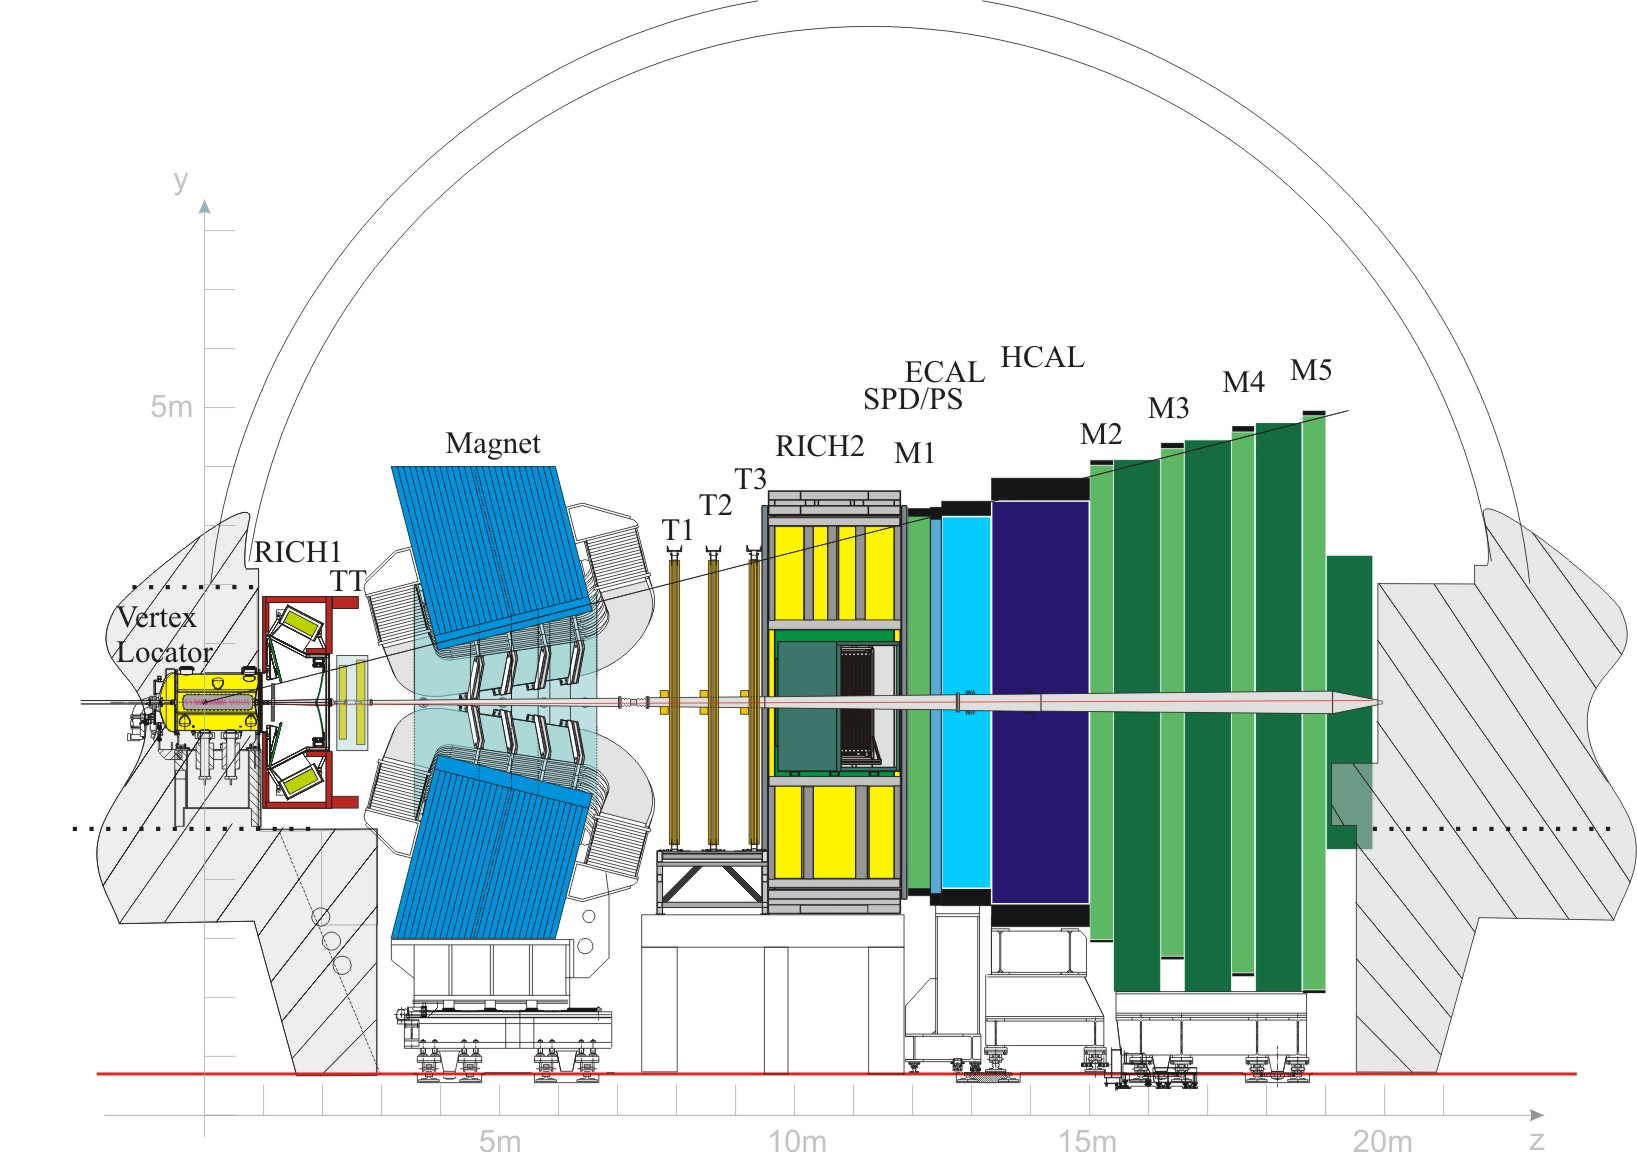
\includegraphics[width=\textwidth,trim=3em 0 0 0,clip]{lhcb.pdf}
      \begin{itemize}
        \item Vorwärts-Spektrometer entwickelt zur Untersuchung schwerer Quarks
      \end{itemize}
    \end{column}
  \begin{column}{0.35\textwidth}
    \begin{itemize}
      \item Gute Stoßparameter-Auflösung: \SI{20}{\micro\metre}
      \item Auflösung der invarianten Masse: \SI{8}{MeV} ($B\to J\!/\!\psi \phi$)
      \item Exzellente Teilchenidentifikation: \SI{95}{\percent} Kaon ID-Effizienz gegen \SI{5}{\percent}
      \item Flexibler Trigger
    \end{itemize}
  \end{column}
  \end{columns}
\end{frame}

%\begin{frame}{Evans et al.}
%  \begin{itemize}
%    \item Use effective field theory approach to separate decay into short/long distance interactions
%    \item In absence of lattice QCD calculations, matrix elements $β$ and $β_8$ are approximated
%    \item BR for $B^0\to D^{(*)0}e^+e^-$ is calculated
%    \item Also give predictions for $B^+\to D_{\!(s)}^{\ (*)+}e^+e^-$ (smaller BR) in a different paper
%    \item Use these to get an idea of expected yields
%  \end{itemize}
%\end{frame}
%
%\begin{frame}{Kim et al.}
%  \begin{itemize}
%    \item Perturbative QCD approach
%    \item Make use of model-dependent wave functions to derive result
%    \item No mention of calculation by Evans et al.
%    \item We should treat this optimistic result with care
%  \end{itemize}
%\end{frame}

\begin{frame}{Wie viele Zerfälle kann man bei LHCb erwarten?}
  \begin{equation*}
    N = \mathcal{L}\,\sigma_{b\overline{b}}\,2 f_d\,ε\,\text{BR}_B\,\text{BR}_D
  \end{equation*}
  Betrachte Zerfälle der Form $B\to D\mu\mu$:\\
  Welche $D$-Endzustände sollten betrachtet werden?
  \begin{itemize}
    \item Bei LHCb gut zu beobachten:
      \begin{itemize}
        \item $D^{0}\to K^-\pi^+$
        \item $D^+\to K^-\pi^+\pi^+$
        \item $D_s^+\to K^+K^-\pi^+$
        \item $D^{*+} \to D^0\pi^+ \to K^-\pi^+\pi^+$
      \end{itemize}
    \item Schwierig zu beobachten (Photonen):
      \begin{itemize}
        \item $D^{*0} \to D^0\pi^0 \to K^-\pi^+\gamma\gamma$
        \item $D_s^{+*}\to D_s^+\gamma \to K^+K^-\pi^+\gamma$
      \end{itemize}
  \end{itemize}
\end{frame}

\begin{frame}{Wie viele Zerfälle kann man bei LHCb erwarten?}
  Nutze Vorhersagen von Evans et al.
  \vspace{0.5em}

  \centering
  \begin{tabular}{l S S}
    \toprule
    Zerfall & {\text{Vorhergesagtes BR}} & {\text{Erwartete Ereignisse}} \\
    \midrule
    $\mathbf{B^0\!\to\! \overline{D}^0\mu\mu}$ & 2.6e-9 & 1.8 \\
    %$B^0\to \overline{D}^{*0}\mu\mu$ & 1.4e-8 & 6.1 \\
    $B^+\!\to\! D^+\mu\mu$ & 2.5e-12 & 0.41e-2 \\
    $B^+\!\to\! D^{+*}\mu\mu$ & 1.0e-11 & 0.48e-2 \\
    $B^+\!\to\! D_s^+\mu\mu$ & 4.3e-11 & 0.17e-2 \\
    %$B^+\to D_s^{+*}\mu\mu$ & 2.0e-10 & 0.12e-1 \\
    $B_c\!\to\!D_s^+\mu\mu$ & ? & ? \\
    \bottomrule
  \end{tabular}
  \begin{itemize}
    %\item BR $\sim 10^{-7}$ (Ebert et al.)
    \item Außerdem: Viele resonante Moden ($B\!\to\! J\!/\!\psi D$) noch nicht beobachtet
  \end{itemize}
\end{frame}

\begin{frame}{Analysestrategie: $B^0\to \overline{D}^0\mu\mu$}
  \linespread{0.9}
  \begin{tikzpicture}[
      analysis/.style={rectangle,draw,fill=blue!20},
      line width=1.2pt,
      align=center,
      node distance=0.5cm]

      \node[text width=11em,analysis] (collision) at (0,0) {Kollision};
      \node[text width=11em,analysis,below=of collision] (trigger) {Trigger};
      \node[text width=11em,analysis,below=of trigger] (stripping) {Vorselektion};
      \node[text width=11em,analysis,below=of stripping] (vorselektion) {Massenvetos/PID};
      \node[text width=11em,analysis,below=of vorselektion] (multivariat) {Finale Analyse-Selektion};
      \node[text width=11em,analysis,below=of multivariat] (fit) {Bestimmung des Limits};

      \uncover<1->{
      \node[node distance=1.5cm,right=of collision] (collision_text) {\SI{3}{fb^{-1}} Daten bei\\ $\sqrt{s}=7\,\text{und}\,\SI{8}{TeV}$};
      \draw[-] (collision.east) -- (collision_text.west);
      }

      \uncover<2->{
      \node[below=of collision_text] (trigger_text) {Muon- und Dimuon-\\ Kandidaten};
      \draw[-] (trigger.east) -- (trigger_text.west);
      }

      \uncover<3->{
      \node[below=of trigger_text] (stripping_text) {Generische Vorselektion\\ von $K^+\pi^-\mu^+\mu^-$};
      \draw[-] (stripping.east) -- (stripping_text.west);
      }

      \draw[->] (collision.south) -- (trigger.north);
      \draw[->] (trigger.south) -- (stripping.north);
      \draw[->] (stripping.south) -- (vorselektion.north);
      \draw[->] (vorselektion.south) -- (multivariat.north);
      \draw[->] (multivariat.south) -- (fit.north);

      \uncover<4->{
      \draw[red,thick] ($(vorselektion.north west)+(-0.2,0.2)$)  rectangle ($(fit.south east)+(0.2,-0.2)$);
      \node[below=of stripping_text] (more_text) {Mehr Details im Folgenden};
      \draw[-,color=red] ($(fit.south east)+(0.2,+1)$) -- (more_text.west);
      }
  \end{tikzpicture}
  \linespread{1.3}
\end{frame}

\begin{frame}{Massenvetos: Signalbereich und $J\!/\!\psi$-Resonanz}
  \centering
  \includegraphics[width=0.45\textwidth]{../../../plots/b_mass.pdf}
  \includegraphics[width=0.45\textwidth]{../../../plots/mumu_mass.pdf}

  \begin{itemize}
    \item Messung soll blind durchgeführt werden: Schnitt auf $B^0$-Masse
    \item Ausschluss von $J\!/\!\psi$ durch Schnitt auf $m(\mu\mu)$
    \item Phasenraum endet bei $m(\mu\mu)\approx \SI{3.4}{GeV}$ $\Rightarrow$ Weiterer Schnitt
  \end{itemize}
\end{frame}

\begin{frame}[shrink=10]{Vorselektion}
  \begin{itemize}
    \item {\small Schnitte auf Teilchenidentifikations-Variablen um Kaon/Pion zu selektieren:}
  \end{itemize}
  \centering
  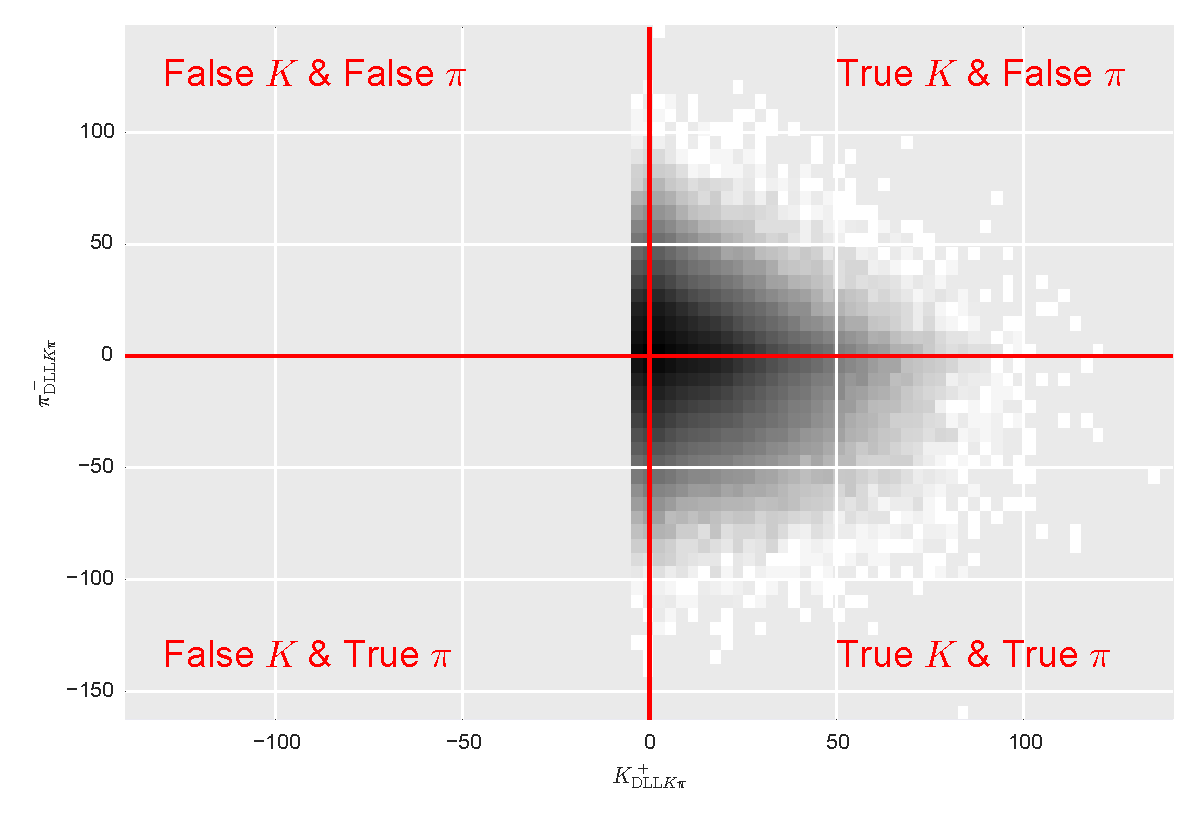
\includegraphics[width=0.65\textwidth]{../../../plots/pid_plot.pdf}
  \begin{itemize}
    \item Wird gemeinsam mit multivariater Selektion optimiert
  \end{itemize}
\end{frame}

\begin{frame}{Multivariate Selektion}
  \begin{itemize}
    \item Klassifizierer: Adaboosted Decision Tree
    \item Nutze Signal-Simulation und oberes Massen-Seitenband als Trainingsgrundlage
    \item Variablen: TODO Liste der wichtigsten Variablen
  \end{itemize}
  TODO: Plots der wichtigsten Variablen auf Signal/Untergrund
\end{frame}

%\begin{frame}[shrink=20]{Multivariate selection: cross-validation, ROC curves}
%  \begin{itemize}
%    \item Use $k$-fold validation to assess quality of classifier (BDT)
%    \item ROC curves for each of the $k=5$ test samples
%  \end{itemize}
%  \centering
%  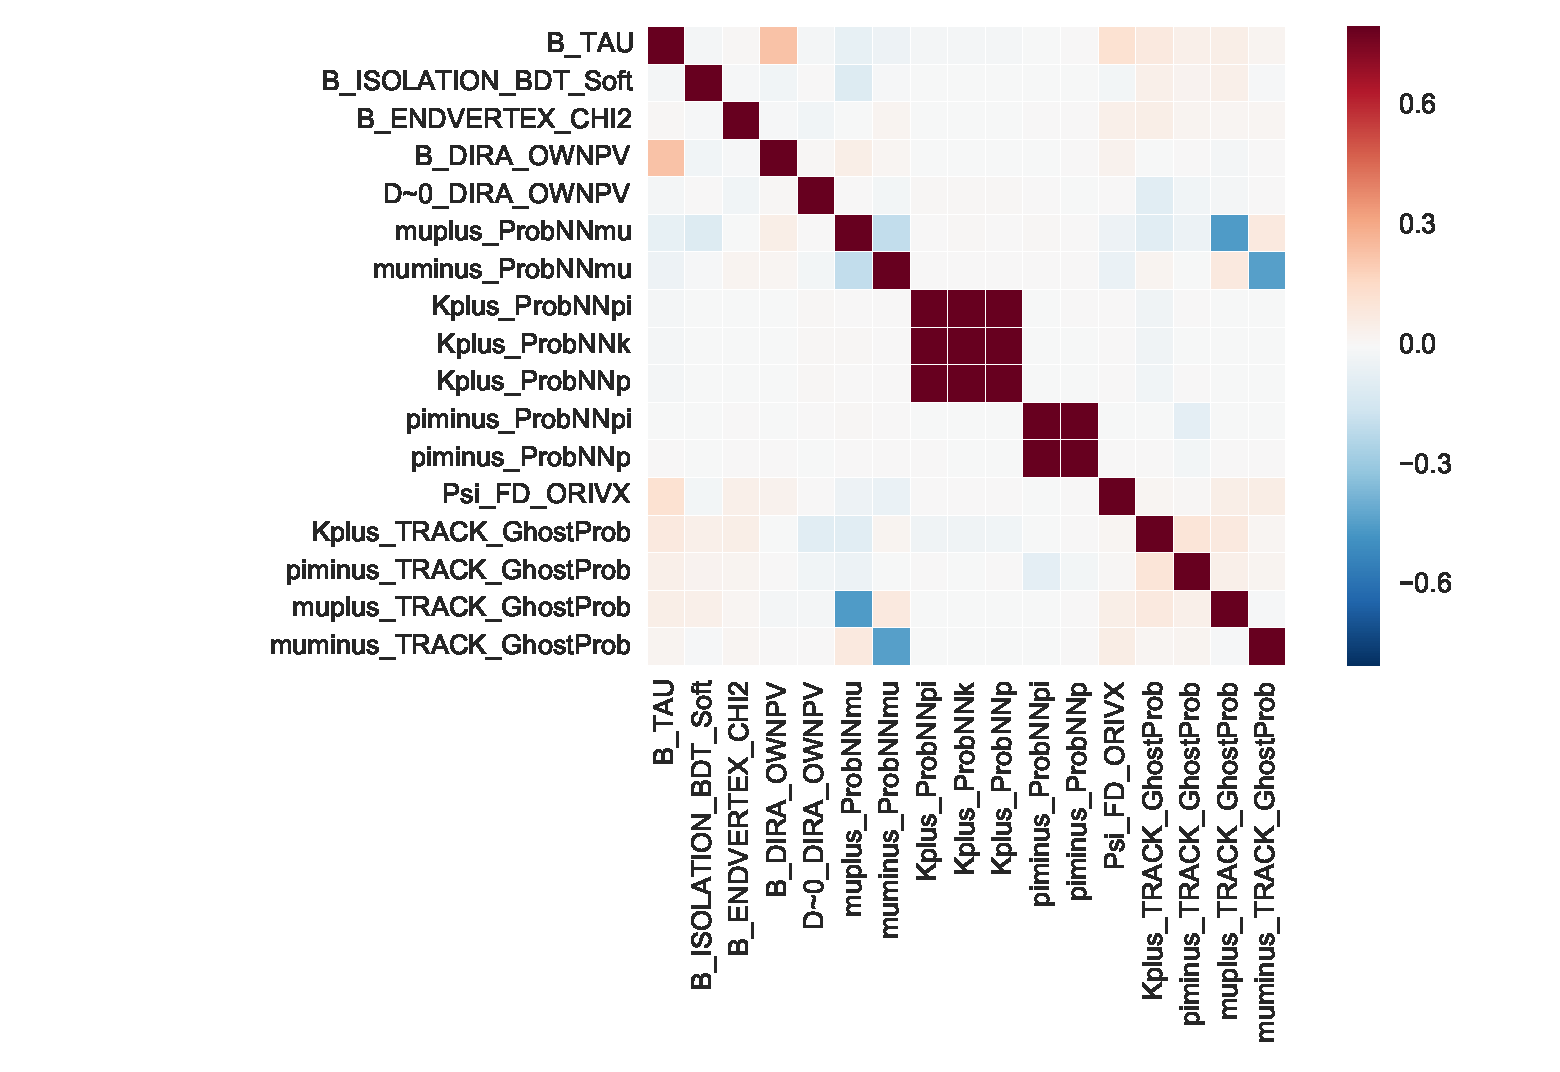
\includegraphics[width=0.50\textwidth,page=1]{../../../plots/classifier.pdf}
%  \includegraphics[width=0.50\textwidth]{../../../plots/classifier_mass.pdf}
%\end{frame}

\begin{frame}[shrink=10]{Nach Selektion: Physikalische Untergründe}
  \begin{itemize}
    \item Kombinatorischer Untergrund effektiv reduziert
    \item \textbf{Aber:} Genaue Kenntnis der physikalischen Untergründe notwendig
  \end{itemize}
  
  {\small Kanal $B^0\!\to\! \overline{D}^0 J\!/\!\psi$ bereits im Rahmen von [PhysRevD.87.112012] untersucht:}

  \includegraphics[width=\textwidth]{vanya2.pdf}
  \begin{itemize}
    \item Hier: Nichtresonanter Untergrund $B^0\!\to\! K^+\pi^- J\!/\!\psi$
    \item Schnitt auf Lebenszeit des $D^0$ schließt $K^-\pi^+$ aus
    \item Aber: Verlust von Signaleffizienz $> \SI{50}{\percent}$
  \end{itemize}
\end{frame}

\begin{frame}[shrink=10]{Entwicklung des statistischen Modells}
  \begin{itemize}
    \item Idee: Gleichzeitige Beschreibung von $B$-Masse, $D$-Masse und $D$-Lebensdauer
    \item Entwicklung gestützt von Toy-Simulation
    \item Formen von Signal und $B^0\to K^+\pi^-\mu\mu$ lassen sich aus Simulation ableiten
  \end{itemize}
  \centering
  \includegraphics[width=0.5\textwidth]{../../../plots/fit_dmass.pdf}
  \includegraphics[width=0.5\textwidth]{../../../plots/fit_bmass.pdf}
\end{frame}

%\begin{frame}{Measurement of branching fraction}
%  Needed are:
%  \begin{itemize}
%    \item trigger efficiency (use TISTOS on control channel)
%    \item stripping efficiency (Simulation)
%    \item LHCb acceptance efficiency (Simulation)
%    \item preselection efficiency (calibrate PID from data)
%    \item selection efficiency of classifier (cross-validation)
%  \end{itemize}
%  $\Rightarrow$ Use signal yield and efficiencies to derive BR estimate.
%  \begin{itemize}
%    \item Choose normalization/control channel:
%      \begin{itemize}
%        \item $B^0\to K^{*0}\mu^+\mu^-$ $\Rightarrow$ Similar behaviour
%        \item $B^0 \to K^{*0}J\!/\!\psi$ $\Rightarrow$ Larger statistics
%      \end{itemize}
%  \end{itemize}
%\end{frame}

\begin{frame}{Ausblick}
  \begin{itemize}
    \item Suche nach $B\!\to\! D \mu^+\mu^-$-Zerfällen in LHCb-Daten begonnen
    \item Zerfälle, die betrachtet werden können:
    \begin{itemize}
      \item $B^0\!\to\!\overline{D}^0\mu\mu$ (momentan untersucht)
      \item $B_c^+\!\to\! D_s^+\mu\mu,\ \  B^+\!\to\! D^{*+}\mu\mu,\ \ B^+\!\to\! D_s^{+}\mu\mu$
      \item Resonante Moden (z.B. $B^0\!\to\! J\!/\!\psi \overline{D}^0$)
    \end{itemize}
  \end{itemize}
  Nach Vorhersage von Evans: Setzen von oberen Schranken erwartet
\end{frame}

\appendix
\beginbackup

\begin{frame}
  \centering
  \Huge Anhang
\end{frame}

\begin{frame}[shrink=20]{Wie wurden die erwarteten Ereigniszahlen ermittelt?}
  \begin{equation*}
    N = \mathcal{L}\,\sigma_{b\overline{b}}\,2 f_d\,ε\,\text{BR}_B\,\text{BR}_D
  \end{equation*}
  \begin{itemize}
    \item $\text{BR}_B$: Vorhersagen von Evans et al.
    \item $\text{BR}_D$: Aus PDG entnommmen:
    \begin{itemize}
      \item $\mathrm{BR}(D^{0}\to K^-\pi^+) = \SI{3.87 \pm 0.05}{\percent}$
      \item $\mathrm{BR}(D^+\to K^-\pi^+\pi^+) = \SI{9.13 \pm 0.19}{\percent}$
      \item $\mathrm{BR}(D_s^+\to K^+K^-\pi^+) = \SI{5.49 \pm 0.27}{\percent}$
      \item $\mathrm{BR}(D^{*0} \to D^0\pi^0) = \SI{61.9 \pm 2.9}{\percent}$
      \item $\mathrm{BR}(D^{*+} \to D^0\pi^+) = \SI{67.7 \pm 0.5}{\percent}$
      \item $\mathrm{BR}(D_s^{+*}\to D_s^+\pi^0) = \SI{5.8 \pm 0.7}{\percent}$
    \end{itemize}
    \item $\mathcal{L} = \num{3.189}(\SI{1.000\pm0.035}{\per\femto\barn})$ [arxiv:1110.2866]
    \item $σ_{b\overline{b}} = 295 \pm 29\,\si{\micro\barn}$
    \item $f_d \approx \num{0.4}$
    \item $ε\approx \SI{2.5}{\percent}$
  \end{itemize}
\end{frame}

\begin{frame}{Test for overfitting}
  \centering
  \includegraphics[width=0.7\textwidth,page=2]{../../../plots/classifier.pdf}
\end{frame}
\backupend

\end{document}

